\documentclass[10pt]{beamer}

\usetheme{metropolis}
\usepackage{appendixnumberbeamer}

\usepackage{booktabs}
\usepackage[scale=2]{ccicons}

\usepackage{pgfplots}
\usepgfplotslibrary{dateplot}

\usepackage{xspace}
\newcommand{\themename}{\textbf{\textsc{metropolis}}\xspace}

\title{Detecting Malicious Shell Commands}
\subtitle{A review of text classification techniques}
\date{\today}
\author{rdube}
% \institute{Center for modern beamer themes}
% \titlegraphic{\hfill\includegraphics[height=1.5cm]{logo.pdf}}


\begin{document}

\maketitle

\begin{frame}{Table of contents}
  \setbeamertemplate{section in toc}[sections numbered]
  \tableofcontents[hideallsubsections]
\end{frame}

\section{Motivation}

\begin{frame}[fragile]{Why study this topic?}
	Several reasons to study the topic:
	\begin{itemize}
		\item PowerShell increasingly used in attacks \cite{symc2016}
		\item (In general) Fileless attack techniques increasing \cite{symc2017}
		\item Scripts becoming weapons of choice for sophisticated attack groups \cite{msft2017-2}
		\begin{itemize}
			\item Fileless technques used during the SolarWinds hack \cite{zdnet2021}
		\end{itemize}
		\item Complicated and obfuscated scripts difficult for human analysts to decipher \cite{feye2018}
	\end{itemize}
\end{frame}

\section{Binary command line model design considerations}

\begin{frame}[fragile]{Major decision points}
	\begin{itemize}
		\item Input data source
		\item Classifier design
	\end{itemize}

	The model design space (under the above headings) is large \cite{survey2021,msft2017,powershell2018,amsi2019,feye2018,feye2018-2,textcnn2016,textcnn2019}:
\end{frame}

\begin{frame}{Input data source considerations...}
	Techniques used, models created may be different based on input assumed \cite{msft2017-2,msft2019,feye2018}:
	\begin{itemize}
		\item PowerShell vs. VBScript vs. Javascript code 
		\item Single command line vs. multi-line script
		\item Raw script vs. that obtained through AMSI or sandbox (if different from raw)
		\item Obfuscated vs. de-obfuscated script
		\item Additional unlabeled corpus of scripts
	\end{itemize}
\end{frame}

\begin{frame}{Classifier design considerations...}
	\begin{itemize}
		\item Token-based features vs. character-based features
		\begin{itemize}
			\item For token-based features
			\begin{itemize}
				\item Encoding (bag-of-words) vs. embedding
				\item Inline embedding vs. externally learned embedding
				\item Word2Vec vs. FastText vs. something else
			\end{itemize}
			\item For character-based features
			\begin{itemize}
				\item Encode each character (bag-of-characters) vs something else
			\end{itemize}
		\end{itemize}
		\item Manual-feature extraction vs. automatic feature extraction
		\begin{itemize}
			\item For automatic feature extraction
			\begin{itemize}
				\item CNN vs. self-attention (to extract features from a segment of the command line)
				\item LSTM vs. position-encoding (to combine signals from sequences of features)
			\end{itemize}
		\end{itemize}
		\item Ensembling technique
		\begin{itemize}
			\item Combine output of individual classifiers vs. combine classifiers inline (i.e., train classifiers together)
		\end{itemize}
	\end{itemize}
\end{frame}

\begin{frame}{Other considerations: what pre-processing to assume?}
	Prior work raises several quesions regarding pre-processing data \cite{powershell2018,amsi2019,feye2018}:
	\begin{itemize}
		\item Mechanism to declare a label malicious?
		\item De-obfuscate script coded in base64 (and other) encodings?
		\item Normalize scripts using different IP addresses?
		\item Normalize scripts using random file names?
		\item Normalize abbreviations?
		\item What demarcation to use between tokens?
		\item Eliminate rare tokens?
		\item De-duplicate scripts via clustering and representative selection?
	\end{itemize}
	But, pre-processing partially depends on the the type of model chosen
\end{frame}

\section{Understanding prior work on malicious command line detection}

\begin{frame}[fragile]{Extract coherent lego blocks}
	\begin{itemize}
		\item textCNN classifier \cite{textcnn2016,textcnn2019,powershell2018}
		\item CNN-LSTM classifier \cite{amsi2019}
		\item textCNN + CNN-LSTM classifier \cite{amsi2019}
		\item Obfuscation detector \cite{feye2018}
	\end{itemize}
\end{frame}

\begin{frame}{Lego block 1: textCNN (1)}
	\begin{figure}
		\includegraphics[scale=0.28]{textcnn}
		\caption{Text CNN model as used in \cite{powershell2018}}
	\end{figure}
\end{frame}

\begin{frame}{Lego block 1: textCNN (2)}
	Classifier design:
	\begin{itemize}
		\item Character encoding (bag-of-characters)
		\item CNN to extract features
		\item No explicit mechanism to learn from sequence
	\end{itemize}
\end{frame}

\begin{frame}{Lego block 2: CNN-LSTM (1)}
	\begin{figure}
		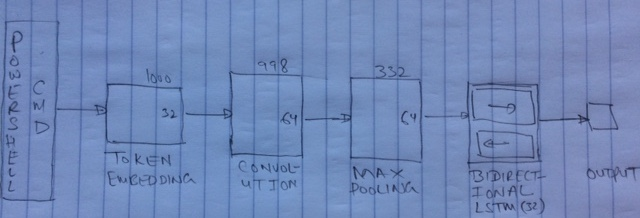
\includegraphics[scale=0.50]{cnn-lstm}
		\caption{CNN-LSTM model as used in \cite{amsi2019}}
	\end{figure}
\end{frame}

\begin{frame}{Lego block 2: CNN-LSTM (2)}
	Classifier design:
	\begin{itemize}
		\item Token based
		\begin{itemize}
			\item FastText embeding from tokens
			\item Externally learned embedding
		\end{itemize}
		\item CNN to extract features
		\item LSTM to learn from sequence of features
		\begin{itemize}
			\item Difficult to parallelize training
		\end{itemize}
	\end{itemize}
\end{frame}

\begin{frame}{Lego block 3: textCNN + CNN-LSTM (1)}
	\begin{figure}
		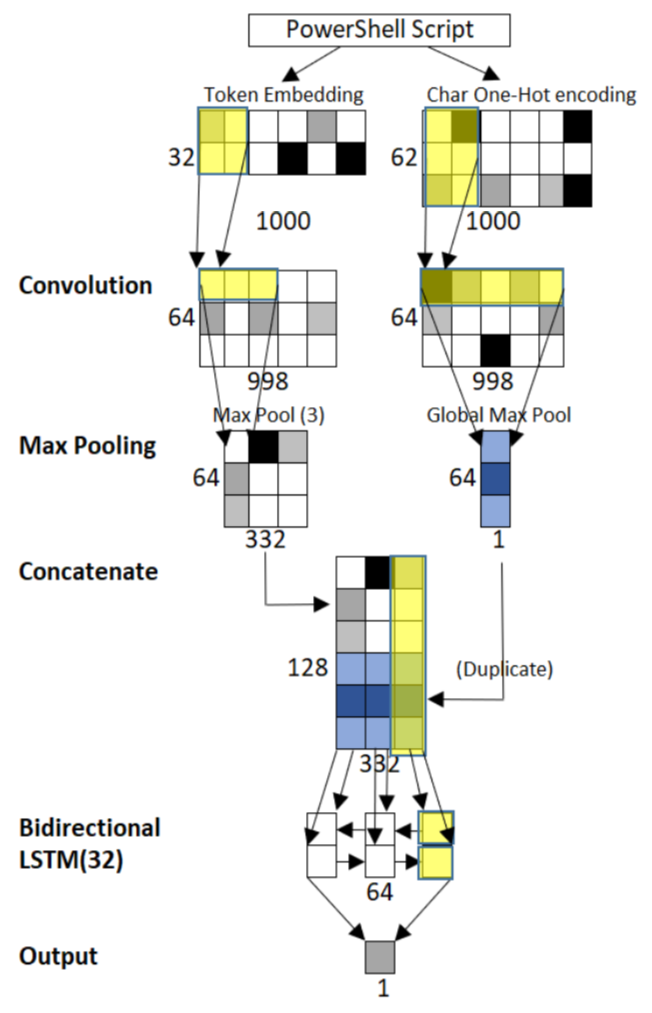
\includegraphics[scale=0.20]{inlineEnsemble}
		\caption{textCNN + CNN-LSTM model as used in \cite{amsi2019}}
	\end{figure}
\end{frame}

\begin{frame}{Lego block 3: textCNN + CNN-LSTM (2)}
	Classifier design:
	\begin{itemize}
		\item Inline ensemble of textCNN and CNN-LSTM
		\item Bi-directional LSTM combines the signals from the two models
	\end{itemize}
	Other notes:
	\begin{itemize}
		\item True positive rate = 0.894 (for false positive rate $\le 10^{-3}$
		\item Embedding training time = 14 hours, Classifier training time = 5 hours
		\begin{itemize}
			\item Unlabeled dataset: 368K PowerShell scripts
			\item Labeled dataset: 117K scripts (5K malicous)
			\item Azure-hosted Data-Science-VM with 56 GB of CPU memory (6 vCPUs) and 12 GB of GPU memory (single core)
		\end{itemize}
	\end{itemize}
\end{frame}

\begin{frame}{Lego block 4: obfuscation detector (1)}
	\begin{figure}
		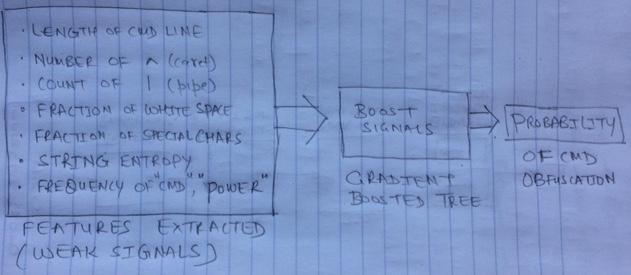
\includegraphics[scale=0.50]{gbtree}
		\caption{Obfuscation detection model as used in \cite{feye2018}}
	\end{figure}
\end{frame}

\begin{frame}{Lego block 4: obfuscation detector (2)}
	Classifier design:
	\begin{itemize}
		\item No expliciting encoding or embedding
		\item Manually extracted features
		\item Tradional machine learning classification technique (gradient boosted trees)
	\end{itemize}
	Other notes:
	\begin{itemize}
		\item Classifier as described, detects obfuscation (not maliciousness)
	\end{itemize}
\end{frame}

\begin{frame}[standout]
  Questions?
\end{frame}

\appendix

\begin{frame}[allowframebreaks]{References}

  \setbeamertemplate{bibliography item}{\insertbiblabel}
  \bibliography{cmd}
  \bibliographystyle{alpha}

\end{frame}

\end{document}
